\documentclass[tikz,border=5pt]{standalone}
\usepackage{amsmath,amssymb}
\usetikzlibrary{arrows.meta,positioning}
\definecolor{curveblue}{HTML}{245C86}
\definecolor{accent}{HTML}{A65E2E}
\begin{document}
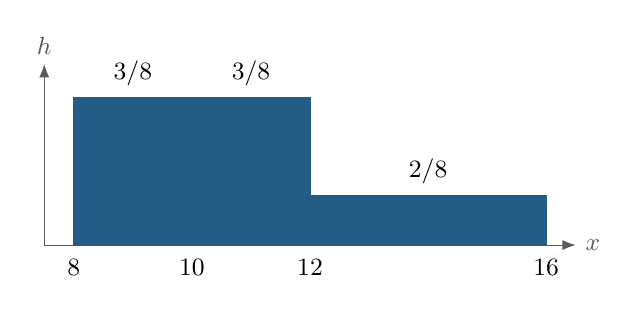
\begin{tikzpicture}[font=\small,>=Latex,line cap=round,line join=round]
\begin{scope}[x=.75cm,y=10cm]
\draw[->,black!65] (7.50000,0.00000)--(16.50000,0.00000) node[right]{$x$};
\draw[->,black!65] (7.50000,0.00000)--(7.50000,0.23000) node[above]{$h$};
\draw[fill=curveblue!15,curveblue] (8.00000,0.00000) rectangle (10.00000,0.18750);
\draw[fill=curveblue!15,curveblue] (10.00000,0.00000) rectangle (12.00000,0.18750);
\draw[fill=curveblue!15,curveblue] (12.00000,0.00000) rectangle (16.00000,0.06250);
\node[below] at (8.00000,-0.00600) {$8$};
\node[below] at (10.00000,-0.00600) {$10$};
\node[below] at (12.00000,-0.00600) {$12$};
\node[below] at (16.00000,-0.00600) {$16$};
\node[above] at (9.00000,0.19000) {$3/8$};
\node[above] at (11.00000,0.19000) {$3/8$};
\node[above] at (14.00000,0.06500) {$2/8$};
\end{scope}
\end{tikzpicture}
\end{document}
